\documentclass[class=report,crop=false, 12pt]{standalone}
\usepackage[screen,nosolutions]{../scratch}

\begin{document}

\titre[S]{Créer ses blocs}
%===============================

\insertvideo{ZUv9GknyERI}{Créer ses blocs -- Activité 1}

\insertvideo{_nYZsBAmM1Q}{Créer ses blocs -- Activité 2}

\insertvideo{aDGl-e-VliU}{Créer ses blocs -- Activité 3}

\bigskip
\bigskip

\emph{Créer ses propres blocs a plusieurs avantages : cela évite de recopier du code qui apparaît plusieurs fois, et le code devient plus court. Le programme ne sera pas plus rapide et le résultat sera le même, mais le code sera plus facile à écrire et à lire !}

\bigskip
\bigskip


\begin{activite}

\sauteligne

\begin{center}
  \includegraphics[scale=\scaleecran]{ecran-11-ex1} 
\end{center}

\begin{enumerate}
  \item Crée ton bloc \codeinline{etoile} qui effectue les instructions suivantes :
    \begin{itemize}
      \item stylo en position d'écriture,
      \item répéter $5$ fois : avancer de $50$, tourner de $216$\textdegree,
      \item relever le stylo.
    \end{itemize}



  \item Dessine une étoile à chaque coin de l'écran. Tu peux changer la couleur et la taille du stylo.
  
  \item Crée un nouveau bloc \codeinline{etoilebis} qui trace une étoile, mais avec la taille que l'on souhaite. Pour cela, le bloc dépend cette fois d'un nombre (que l'on peut appeler \codeinline{taille} par exemple) et, au lieu d'avancer de $50$, on avance de \codeinline{taille}.
  
  \item Trace des étoiles de taille $30$, $40$, $50$... au centre de l'écran.
\end{enumerate}

\bigskip

\textbf{Blocs utiles.}
Crée tes propres blocs dans la catégorie \og Ajouter blocs \fg{}, puis \og Créer un bloc \fg{}. Donne lui un nom bien choisi, et dans les options on peut ajouter des paramètres.  

\begin{center}
  \includegraphics[scale=\scalebloc]{bloc-11-ex1} 
\end{center}

\end{activite}


\begin{activite}

Les \emph{effets moirés} sont des formes qui apparaissent lors du tracé  de formes géométriques simples sur un écran. La figure du haut est uniquement constituée de cercles, celle du bas de segments.

\begin{center}
  \includegraphics[scale=\scaleecran,scale=0.8]{ecran-11-ex2a} 
\end{center}
\begin{center}  
  \includegraphics[scale=\scaleecran,scale=0.8]{ecran-11-ex2b}   
\end{center}

\begin{enumerate}
  \item Crée un bloc \codeinline{cercle} qui exécute les instructions suivantes :
    \begin{itemize}
      \item stylo en position d'écriture,
      \item répéter $30$ fois : avancer de $15$, tourner de $12$\textdegree,
      \item relever le stylo.
    \end{itemize}  

  \item Trace des centaines de cercles, en avançant de quelques pas à chaque fois (figure du haut).
  
  \item Crée un bloc \codeinline{droite} qui dépend d'un nombre
 \codeinline{valy} et qui trace une droite du point $(-200,0)$ au point $(200,\text{\codeinline{valy}})$. Les instructions sont les suivantes :
    \begin{itemize}      
      \item relever le stylo,
      \item aller à $(-200,0)$,
      \item stylo en position d'écriture,
      \item aller à $(200,\text{\codeinline{valy}})$.
    \end{itemize}   
  
  \item Définis une variable $y$. Fais varier $y$ entre $-150$ et $+150$ de façon à tracer beaucoup de droites grâce au bloc \codeinline{droite} $(y)$ (figure du bas).  
    
\end{enumerate}
  
\end{activite}



\begin{activite}

Les dessins suivants ont été réalisés à partir de figures simples.

\begin{center}
  \includegraphics[scale=\scaleecran]{ecran-11-ex3} 
\end{center}

\begin{enumerate}
  \item Le dessin en haut à gauche est obtenu par les instructions suivantes.
\begin{center}
  \includegraphics[scale=\scalebloc]{bloc-11-ex3a} 
\end{center} 

\`A toi de définir le bloc \codeinline{carre}.


  
  \item Le dessin en haut à droite est obtenu par les instructions suivantes.
\begin{center}
  \includegraphics[scale=\scalebloc]{bloc-11-ex3b} 
\end{center} 

\`A toi de définir le bloc \codeinline{triangle} ayant un argument.

   
 
  \item Le dessin du bas est obtenu par les instructions suivantes.
\begin{center}
  \includegraphics[scale=\scalebloc]{bloc-11-ex3c} 
\end{center} 

\`A toi de définir le bloc \codeinline{segment} ayant deux arguments.
  
  
\end{enumerate}
  
\end{activite}


\ifx \displaysolutions \myzero
\else
\begin{code}
\onesolution{Créer ses blocs}{Activité 1}{\includegraphics[scale=\scalesolution]{code-11-ex1}}
\onesolution{Créer ses blocs}{Activité 2}{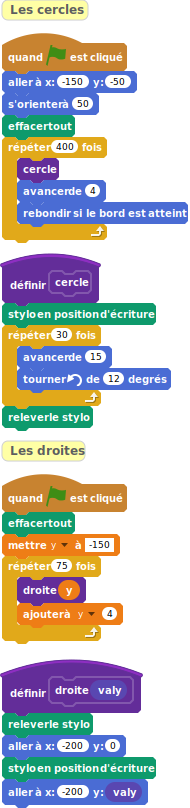
\includegraphics[scale=\scalesolution]{code-11-ex2}}

\onesolution{Créer ses blocs}{Activité 3}{
\includegraphics[scale=\scalesolution,scale=0.7]{code-11-ex3a}
\includegraphics[scale=\scalesolution,scale=0.7]{code-11-ex3b}
\includegraphics[scale=\scalesolution,scale=1]{code-11-ex3c}
}    
\end{code}
\fi


\end{document}
